\documentclass[letterpaper, 12pt]{article}
\usepackage[a4paper, total={6.5in, 10in}]{geometry}
\usepackage{svg}
\usepackage{tikz}
\usetikzlibrary{shapes.geometric, arrows}
\usepackage{float}
\usepackage{lipsum}
\usepackage{animate}
\usepackage{wrapfig}
\usepackage{environ}
\usepackage{amsmath}
\usepackage{listings}
\usepackage{algpseudocode}
\usepackage{algorithm}
\usepackage{graphicx}
\usepackage{hyperref}
\usepackage{tabularx}
\usepackage{nicematrix}
\usepackage{booktabs}
\usepackage{enumitem}
\svgpath{ {./images/} }
\graphicspath{ {./images/} }
\floatstyle{boxed}

\tikzstyle{startstop} = [rectangle, rounded corners, minimum width=3cm, minimum height=1cm,text centered, draw=black, fill=red!30]
\tikzstyle{io} = [trapezium, trapezium left angle=70, trapezium right angle=110, minimum width=3cm, minimum height=1cm, text centered, draw=black, fill=blue!30]
\tikzstyle{process} = [rectangle, minimum width=3cm, minimum height=1cm, text centered, draw=black, fill=orange!30]
\tikzstyle{framework} = [rectangle, minimum width=3cm, minimum height=1cm, text centered, draw=black, fill=cyan!30]
\tikzstyle{decision} = [diamond, minimum width=3cm, minimum height=1cm, text centered, draw=black, fill=green!30]
\tikzstyle{arrow} = [thick,->,>=stealth]

\algnewcommand\algorithmicforeach{\textbf{for each}}
\algdef{S}[FOR]{ForEach}[1]{\algorithmicforeach\ #1\ \algorithmicdo}

\title{
  \includegraphics[width=2cm]{unipi_logo.png}\\[1cm]
  Applications of The NEAT Algorithm in Deterministic Game Environments
}
\date{\today}
\author{John Kechagias\\ Department of Informatics, University Of Piraeus}

\makeatletter
\newsavebox{\measure@tikzpicture}
\NewEnviron{scaletikzpicturetowidth}[1]{%
  \def\tikz@width{#1}%
  \def\tikzscale{1}\begin{lrbox}{\measure@tikzpicture}%
  \BODY
  \end{lrbox}%
  \pgfmathparse{#1/\wd\measure@tikzpicture}%
  \edef\tikzscale{\pgfmathresult}%
  \BODY
}
\makeatother
\begin{document}

\maketitle

\begin{abstract}
This paper explores the use of the NEAT algorithm combined with self-play in
deterministic game environments. Our objective is to investigate how quickly models can
adopt specific strategies with minimal reliance on training data and expert knowledge.
We developed a game similar to the board game Catan as a platform for training models.
Multilayer feedforward neural networks were used to evaluate board positions, and games
were played using a minimax search strategy. In each generation, neural networks
competed against the best networks from the previous generation. Poorly performing
networks were eliminated, and the survivors produced offspring through crossover and
mutation.

\parskip=0.5cm

\noindent\textbf{Keywords:} Artificial Neural Networks · NEAT algorithm · Deterministic
Game Environments · Self-play
\end{abstract}

\section{Introduction}
In recent years, the field of artificial intelligence has seen significant advancements
in training models to perform complex tasks, particularly within game environments. One
promising approach in this domain is the NeuroEvolution of Augmenting Topologies (NEAT)
algorithm \cite{stanley:ec02}, which evolves neural networks by adjusting both their
weights and topologies. A key advantage of NEAT is its ability to avoid getting trapped
in local optima, enabling the discovery of more effective strategies over time, even on
complicated fitness landscapes. When combined with self-play, where agents learn by
playing against themselves, NEAT shows great potential for training agents in a variety
of strategic games.

This paper investigates the efficacy of the NEAT algorithm in combination with self-play
to train agents in deterministic game environments. Our primary objective is to evaluate
the speed and efficiency with which these models can learn specific strategies,
minimizing the need for training data and usage of expert knowledge. To provide a
concrete demonstration of this methodology, we developed a game environment similar to
the board game Catan. This platform allows us to systematically train models to adopt
predefined strategies. By focusing on a deterministic game, we ensure that the outcomes
are solely influenced by the strategies employed, thus providing a clear measure of the
effectiveness of our training approach. We aim to highlight the strengths and potential
limitations of integrating NEAT with self-play through a series of experiments. The
results obtained from our study could help better understand the advantages that NEAT
offers in such environments and lead to the development of more efficient and accessible
methods for training AI agents, not only in games but also in other domains where
strategic decision-making is required.

The paper is structured as follows. Firstly, we introduce the NEAT algorithm and
self-play, providing some context regarding their histories, concepts, and
functionalities. Then, we introduce the game environment utilized. After that, we give
an overview of the training process and the gameplay algorithm used. Finally, we present
the experimental results, followed by the conclusion and future work.

\section{Background}
This section provides an overview of the history of the NEAT and self-play algorithm.

\subsection{Neuroevolution}
Neuroevolution (NE) is a branch of artificial intelligence that utilizes evolutionary
algorithms to produce artificial neural networks \cite{bartz2014, flor2008}, rules and
parameters \cite{neuro19,evo2005,edgar2020}. It is primarily applied to general game
playing (GGP), robot control \cite{sekaj2019} and artificial life \cite{neurogames}.
Drawing inspiration from Darwinism, evolutionary algorithms work by creating successive
generations of neural networks mutating them and then evaluating them. After the
networks have been assessed, the fittest of them are selected for reproduction and
create the next generation, leading to fitter offspring in the long-run. The main
advantage of Neuroevolution is that it only requires a measure of a network's
performance at a task, as it searches for a behaviour instead of a value function. This
has two distinct benefits. Firstly, because neuroevolution does not take into account
the fitness landscape, as opposed to more generally used optimization methods like
gradient descent, it is less likely to get stuck on local minima. Secondly, it does not
require curated datasets of input-output pairs, as opposed to supervised learning
algorithms.

In traditional NE approaches, evolving networks have a predetermined structure that is
chosen before the experiment. This usually corresponds to a single hidden layer where
each neuron is connected to all input and output neurons. By using a fixed layout of
neurons the problem becomes a weight optimization problem where we search through the
weight space for optimal values. However, it isn't always easy to select a good
representation in advance. Firstly, the complexity of the structure should reflect the
complexity of the problem, therefore a singular structure cannot be ideal for all
problems. Secondly, although a single hidden layer is able to represent any function, it
does not mean that every function can be easily represent by one. This can be partially
solved by the addition of subsequent hidden layers, but this grows and complexifies the
search space exponentially. Additionally, the growth of the search space exacerbates the
problem of competing conventions, where different networks correspond to the same
function and crossover leads to damaged offspring. This paradigm of static
representations shifted in the 1990s with the emergence of topology and weight evolving
artificial neural networks (TWEANNs). These new methods introduced new mutations to the
evolutionary process that altered the structure of the networks; for instance, the
addition of a neuron or connection.

\subsection{Neuroevolution of Augmenting Topologies}
One of the most successful TWEANN algorithms is NEAT (Neuroevolution of augmenting
topologies) \cite{stanley:ec02}. Developed by Kenneth O. Stanley and Risto Miikkulainen
in 2002, NEAT borrows a lot of concepts from genetic algorithms \cite{lamangup} and aims
to improve upon its TWEANN predecessors. It provides meaningful crossover of different
topologies through the tracking of the historical origin of genes, protects
underdeveloped innovations through speciation and keeps topologies small by starting
with a minimal structure and incrementally growing it. 

NEAT has proven to be an efficient solution for reinforcement learning problems in
various fields, including network security \cite{zhuka2024}, robot control
\cite{silva2012}, and game development \cite{hasting2009, hind2024}. Enhancements for
the algorithm are continually being developed \cite{ambrosio2014, merrild1017}. NEAT is
particularly successful when the cost function is not easily defined. The algorithm
helps networks avoid local optima and develop diverse strategies by preserving
innovations through speciation based on model similarity. This approach allows networks
time to optimize their new structural innovations, rather than being discarded due to
short-term fitness dips, resulting in species developing distinct strategies.
Furthermore, NEAT only requires a measure of a network's performance, making it
applicable for training models on games without relying on expert knowledge.

NEAT uses a variable-length genetic encoding where each individual (Genome) has a list
of node genes and a list of connection genes:

\begin{itemize}
  \item Node genes represent network nodes. They hold information such as the node type
    (input, output, hidden) as well as its innovation number. 
  \item Connection genes represent the connection between two nodes. They hold
    information such as the input node, output node, connection weight, an enable bit
    (whether or not the gene is expressed) and an innovation number.
\end{itemize}

There are four kinds of generic mutations: two structural mutations, a weight mutation
and a mutation that alters the enable bit. The structural mutations expand the network
by either adding a node between an existing connection or a connection between existing
nodes (see Figures \ref{fig:add_node}, \ref{fig:add_con}). In addition, there is the
common weight mutation present in multiple other such methods where the weight of
connections is either set to a random value, set to a default value or slightly altered
based on a distribution. Finally, there is the mutation that alters the enable bit,
thereby altering the expression of the gene.

\begin{figure}[H]
  \centering
  \includesvg[width=0.9\textwidth]{add_node.svg}
  \caption{Add node mutation.}
  \label{fig:add_node}
\end{figure}

\vspace{1cm}

\begin{figure}[H]
  \centering
  \includesvg[width=0.9\textwidth]{add_connection.svg}
  \caption{Add connection mutation.}
  \label{fig:add_con}
\end{figure}

\subsubsection{Tracking of Genes}
One problem that every genetic algorithm has to deal with the problem of competing
conventions. The problem of competing conventions \cite{schafwhit}, also known as the
Permutations Problem \cite{Radcliffe1993GeneticSR} arises in evolutionary algorithms
when different networks correspond to the same function. During crossover, these
networks are likely to yield offspring that deviate significantly from the original
function, leading to a loss in innovation.

NEAT solves this by using innovation numbers that acts as identifiers for structural
components. An innovation number is an extra property that is attached to genes and
works like an ID. When a structural mutation occurs, it is paired with an innovation
number and saved on an innovation record table. The same innovation number is used as
the ID of the produced gene. New, higher numbers are generated for each additional gene.
Whenever a structural mutation occurs we first check if it has already been registered
on the innovation record table, if it has we make sure to use the same identifiers as
previously. This allows for the same structural component to be identified as the same
across all genomes and generations.

\begin{figure}[H]
    \centering
    \includesvg[width=0.9\textwidth]{innovation_record.svg}
    \caption{
      Structural mutation in NEAT. A node with ID 5 is added between nodes 2 and 4. This
      addition is recorded by adding a new entry in the innovation record, linking the
      mutation of the connection (2,4) with the innovation number 5. Subsequently, if
      the connection (2,4) is mutated in any network the produced node will be assigned
      ID 5. This can also be interpreted as node 5's ancestor being the connection
      (2,4).
    }
\end{figure}

The utilization of innovation numbers not only addresses the problem of competing
conventions, but it also simplifies crossover, as it removes the need for expensive
topological analysis. Crossing over two genomes is done by lining up their innovation
number in chronological order (ascending order). Matching genes are inherited randomly,
whereas nonmatching genes are are inherited from the more fit parent.

\subsubsection{Speciation}
To maximize the solution space covered, a diverse population of varying topologies is
required. Since different topologies evolve at different rates, a mechanism is required
to safeguard them from unfair competition. NEAT addresses this by introducing
speciation. In each generation, genomes are separated into species based on a distance
metric, allowing them to compete primarily within their own niche. The bigger the
distance the more dissimilar the genomes are. The distance is computed by taking into
account the number of genes in the largest genome \(N\), excess \(E\) and disjoint \(D\)
genes, as well as the overage weight differences of matching genes \(\overline{W}\),
including disabled genes:

\[\delta=\frac{c_1E}{N}+\frac{c_2D}{N}+c_3 \cdot \overline{W} \hspace{0.5cm}\text{(2.1)}\]

The hyperparameters \(c_1\), \(c_2\) and \(c_3\) help fine-tune the function. Genomes
whose distance fails below a given threshold can be grouped into the same species.
Subsequently, genomes are assigned to the most similar species. If a genome does fails
to be assigned to a preexisting species it creates a new one. In addition, an explicit
fitness sharing \cite{goldbergarichardson} is employed to make it hard for any species
to grow large enough to take over the entire population. The method works by allotting
each species a number of offspring slots that is proportional to the average fitness of
its members. Within each species, individuals then compete with other for the change to
reproduce. A select number of the fittest individuals reproduce via crossover, while all
the other individuals are discarded. Each population is replaced in its entirety by its
offspring.

\subsubsection{Growing From Minimal Topology}
Many predecessors of NEAT had their initial population be random topologies
\cite{Gru1996,Xin1999}. While this approach ensures topological diversity from the
start, it also introduces optimization problems, as random topologies are bound to have
unnecessary genes that need time to be filtered out. NEAT adopts a different strategy.
By starting with a population of topologies that only include the input and output nodes
it eliminates the extra time required to weed out unnecessary genes and ensures that
only necessary genes are included.

\subsection{Self-Play}
Self-play, a technique where agents learn by competing against variations or copies of
themselves, has emerged as a powerful tool in multi-agent reinforcement learning (MARL)
\cite{5392560}. In this approach, agents train by interacting with copies of themselves,
enabling a gradual escalation of challenge and complexity within the learning
environment. Notably, one major advantage of this technique is its nonnecessity for
training data, thereby eliminating the need for pre-collected datasets. A seminal
contribution to this field is AlphaGo Zero \cite{silver2017mastering}, a model trained
to play the board game Go, which achieved remarkable results against human players by
utilizing a self-play learning schema. In our study, we use an approach similar to that
of AlphaGo Zero. Self-play is employed to enhance our fitness function.

\section{Methodology}
To evaluate NEAT in a deterministic game environment, we created a game similar to the
board game \textbf{Catan}. The idea is to use the NEAT algorithm in conjunction with
self-play to train neural models based on specific game strategies. We monitor and
evaluate their progress, and finally, conduct a live assessment where the best model
faces off against a human opponent. To accomplish this, three components are required:
the custom game itself, an algorithm employing a neural model for gameplay, and a system
for training the neural models using NEAT and self-play.

\subsection{Game Overview}
The game is played on a five by five board with hexadecimal tiles (see Figures
\ref{fig:transfer_move}, \ref{fig:production_move}). There are two players, denoted as
\textbf{red} and \textbf{blue}. Players start on opposite corners of the board with one
piece each. Each board tile can hold a maximum of ten pieces. We say that a player owns
a tile when he has pieces on it. The blue player moves first and then play alternates
between sides. The goal of the game is to eliminate all of the pieces of the opponent.
There are two moves available to each player, \textbf{transfer} and \textbf{production}.
Each board position can be represented as a five by five matrix, where each cell
indicates the number of pieces on the corresponding tile. Positive numbers denote pieces
belonging to the blue player, while negative numbers denote pieces belonging to the red
player.

\subsubsection{Transfer Move}
Players can select any number of their owned pieces from a tile and transfer them to a 
neighbouring tile. For this move to be valid, the following conditions must be met:
\begin{itemize}
  \item The starting tile and the destination tile are adjacent.
  \item The number of selected pieces must not exceed the total number of pieces on the
    starting tile.
  \item The total number of pieces on the destination tile must not exceed the maximum 
    allowed number of pieces on a tile.
\end{itemize}
If the destination tile is occupied by the opposing player, a fight ensues. During the
fight, the number of tiles possessed by the player with the greater quantity is
subtracted from both sides. For example, blue player transfers six pieces from tile
\((4, 0)\) to \((3, 1)\):

\begin{figure}[H]
  \begin{minipage}[c]{.5\textwidth}
    \centering
    \includegraphics[width=0.9\textwidth]{transfer_example_1.png}
    \caption{Before the Transfer Move.}
    \label{fig:transfer_move}
  \end{minipage}%
  \begin{minipage}[c]{.5\textwidth} \centering
    \includegraphics[width=0.9\textwidth]{transfer_example_2.png}
    \caption{After the Transfer Move.}
  \end{minipage}
\end{figure}

If a transfer move results is the capture of enemy pieces then it is also called a
\textbf{capture move}. A transfer move is represented by a tuple consisting of the
coordinates of the source tile, the coordinates of the target tile, and a number
indicating the number of pieces transferred. For example, the transfer of \(10\)
soldiers from tile \((0,1)\) to tile \((1,1)\) is represented as \(((0,1), (1,1), 10)\).

\subsubsection{Production Move}
Players can select a tile they occupy and add one more piece to it. For this move to be
valid, the number of pieces on the tile must be less than the maximum allowed number of
pieces on a tile. For example, blue player produces a piece on tile \((3, 1)\):

\begin{figure}[H]
  \begin{minipage}[c]{.5\textwidth}
    \centering
    \includegraphics[width=0.9\textwidth]{production_example_1.png}
    \caption{Before the Production Move.}
    \label{fig:production_move}
  \end{minipage}%
  \begin{minipage}[c]{.5\textwidth} \centering
    \includegraphics[width=0.9\textwidth]{production_example_2.png}
    \caption{After the Production Move.}
  \end{minipage}
\end{figure}

A production move is represented by a tuple consisting of the coordinates of the source
tile and the coordinates of the target tile. For example, the production of a soldier on
tile \((0,1)\) is represented as \(((0,1), (0,1))\).

\subsection{Gameplay Algorithm}
The gameplay algorithm operates by examining possible moves and countermoves up to a
defined depth, utilizing a neural network to evaluate each resulting game state. These
potential moves form a tree structure, allowing the use of a tree search algorithm to
identify the most advantageous scenario. Since each tree node corresponds to a game
state created by executing the moves leading to the move under evaluation, we can
provide its matrix representation to a neural network. This network assesses the game
state from the perspective of the moving player and assigns it a score. To search
through the move tree, we use the principal variation search (PVS) algorithm, an
enhanced version of alpha-beta pruning \cite{Brud1963}.

\subsection{Move Searching} 
The idea is to search through all the possible moves and countermoves up to a given
depth and utilize the neural network for assessing each game state. The job of the
neural networks is to take the matrix form of a game state as input and output a score
indicating how favourable the position is from the perspective of the player whose
pieces are represented with positive numbers. Since the networks are designed to
evaluate positions only from the perspective of the player with positive pieces, when we
want to evaluate a position from the perspective of a player whose pieces are
represented with negative numbers, we multiply the matrix by \(-1\) to switch
perspectives. 

To summarize, we use principal variation search to explore moves up to the given depth.
Each game state is evaluated by the neural network, and when changing player turns, we
multiply the matrix by \(-1\) to switch perspectives. After completing the search, we
select the move that results in the most advantageous game state for the current player.

\subsubsection{Principal Variation Search}
Before explaining how the principal variation algorithm works, we have to explain the
concept of the principal variation. The principal variation is the sequence of moves
that players determine to be the best possible outcome given their analysis of the
current position. In other words, it is the line of play that both sides believe will
lead to the most advantageous position for them.

The Principal Variation Search algorithm (PVS) \cite{Mar1982} represents an enhancement
of the alpha-beta algorithm. It relies on effective move sorting, as it is structured
around the concept that moves positioned closer to the beginning of the move list are
generally better and more likely to be part of the principal variation. This
prioritization allows the PVS algorithm to save time by primarily exploring moves deemed
to be within the principal variation. By initially probing the most promising paths, PVS
can effectively prune the search tree, discarding less relevant branches \cite{Mar1985}.
Moreover, it operates under the 'fail-soft' principle, meaning that if an earlier move
in the sorted list fails high (produces a cutoff with a value greater than or equal to
beta), subsequent moves are searched with a reduced window around the previous result.
This approach not only accelerates the search process but also enables the algorithm to
focus its efforts on the most promising paths, leading to more accurate evaluations. To
further improve the performance of the algorithm, multiple optimization techniques have
been applied like singular extensions, late move reduction and the utilization of a
transposition table.

\begin{scaletikzpicturetowidth}{\textwidth}
\begin{tikzpicture}[scale=\tikzscale,font=\footnotesize]
\tikzstyle{solid node}=[circle,draw,inner sep=1.5,fill=black]
\tikzstyle{hollow node}=[circle,draw,inner sep=1.5]
\tikzstyle{level 1}=[level distance=15mm,sibling distance=3.5cm]
\tikzstyle{level 2}=[level distance=15mm,sibling distance=1.5cm]
\tikzstyle{level 3}=[level distance=15mm,sibling distance=1cm]
\node(0)[solid node,label=above:{$P1$}]{}
child{node[solid node,label=above left:{$P2$}]{}
child{node[hollow node,label=below:{$(1,2)$}]{} edge from parent node[left]{$C$}}
child{node[hollow node,label=below:{$(1,-1)$}]{} edge from parent node[left]{$D$}}
child{node[hollow node,label=below:{$(0,2)$}]{} edge from parent node[right]{$E$}}
edge from parent node[left,xshift=-5]{$A$}
}
child{node[solid node,label=above right:{$P2$}]{}
child{node[hollow node,label=below:{$(2,2)$}]{} edge from parent node[left]{$F$}}
child{node[hollow node,label=below:{$(1,3)$}]{} edge from parent node[right]{$G$}}
edge from parent node[right,xshift=5]{$B$}
};
\end{tikzpicture}
\end{scaletikzpicturetowidth}

\subsection{Model Training}
For our purposes, a system was developed in Python utilizing the NEAT algorithm and
self-play that allows for the relatively quick training and evaluation of agents. It
allows users to define their own evaluation functions responsible for evaluating the
performance of models based on a game and adjust the process through parameterization.
To address the need for parallel training and evaluation of multiple agents, we have
utilized the built-in multiprocessing module of Python and Numba, a just-in-time (JIT)
Python compiler.

\subsection{NEAT Implementation Overview}
To keep things organized, the implementation of the NEAT
algorithm\footnote{\url{https://github.com/JohnKechagias/neat-proc}} is separated from
the implementation of the training model. The NEAT implementation is written in Python
and is based on the original paper by Stanley and Miikkulainen \cite{stanley:ec02}.
While the core algorithm remains unchanged, we have introduced some modifications such
as elite genomes and interspecies crossover.

\begin{figure}[H]
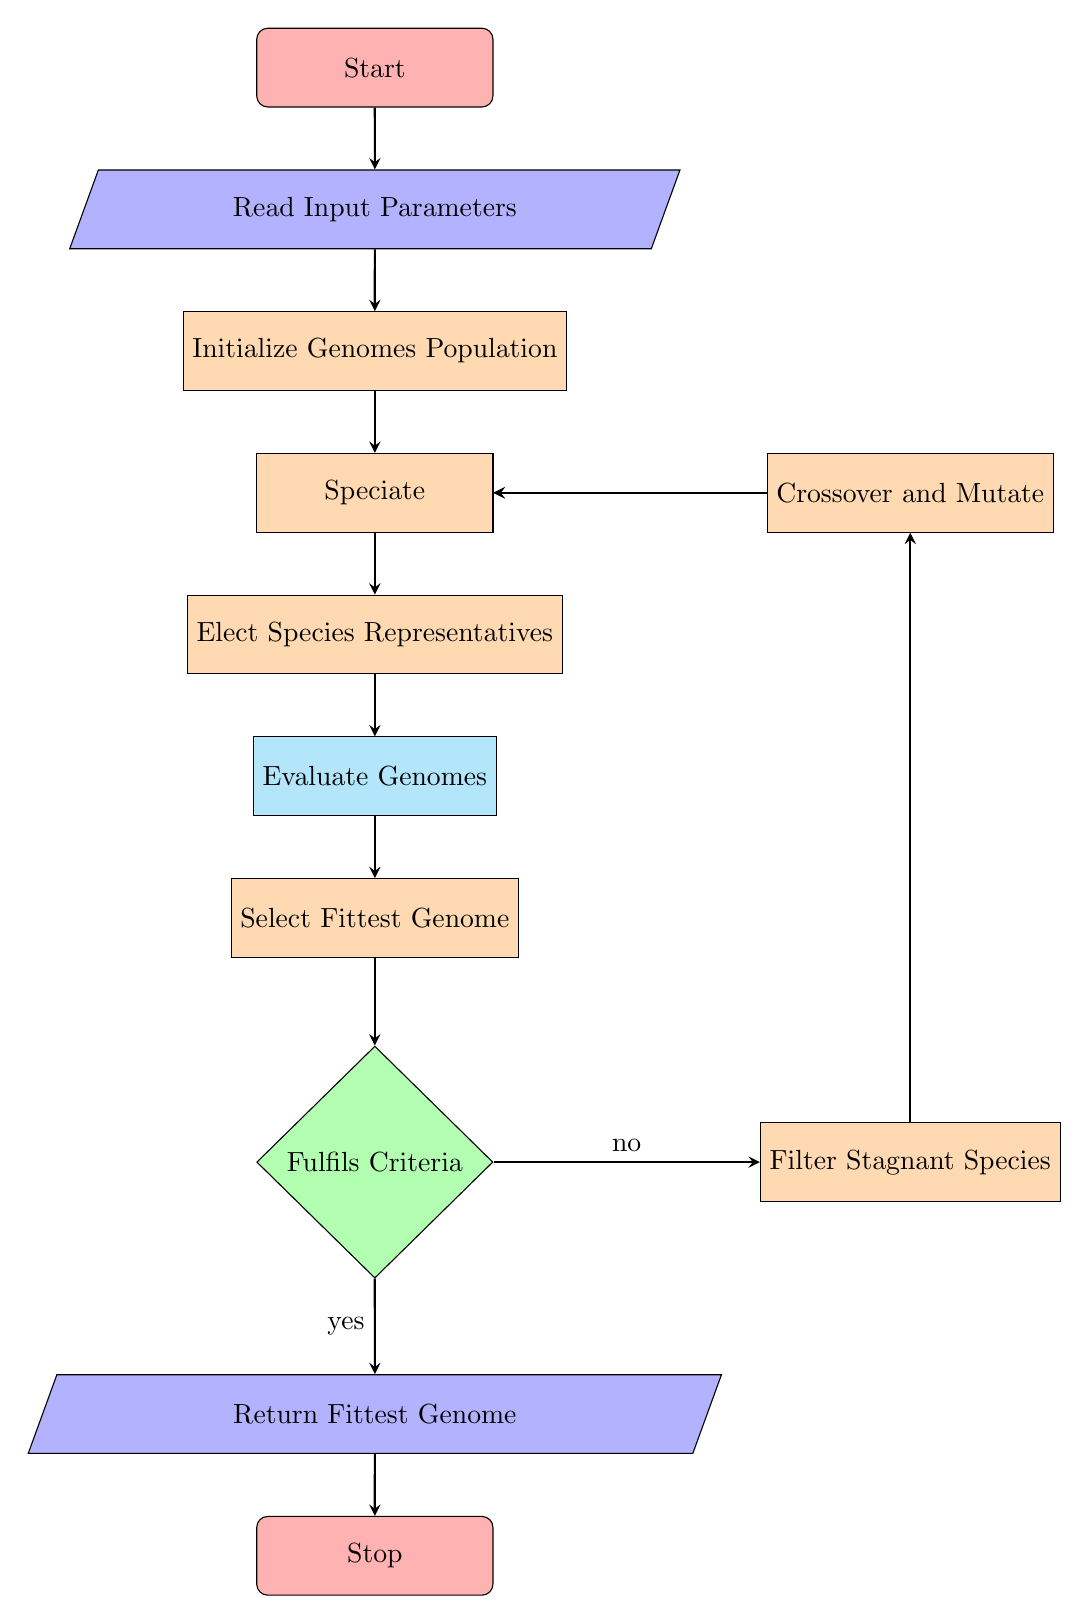
\begin{tikzpicture}[node distance=1.8cm]
\node (start) [startstop] {Start};
\node (read_params) [io, below of=start] {Read Input Parameters};
\node (init_pop) [process, below of=read_params] {Initialize Genomes Population};
\node (speciate) [process, below of=init_pop] {Speciate};
\node (reproduce) [process, right of=speciate, xshift=5cm] {Crossover and Mutate};
\node (select_repr) [process, below of=speciate] {Elect Species Representatives};
\node (evaluate) [framework, below of=select_repr] {Evaluate Genomes};
\node (select_fit) [process, below of=evaluate] {Select Fittest Genome};
\node (fulfils_crit) [decision, below of=select_fit, yshift=-1.3cm] {Fulfils Criteria};
\node (filter_stag) [process, right of=fulfils_crit, xshift=5cm] {Filter Stagnant Species};
\node (return_genome) [io, below of=fulfils_crit, yshift=-1.4cm] {Return Fittest Genome};
\node (stop) [startstop, below of=return_genome] {Stop};

\draw [arrow] (start) -- (read_params);
\draw [arrow] (read_params) -- (init_pop);
\draw [arrow] (init_pop) -- (speciate);
\draw [arrow] (speciate) -- (select_repr);
\draw [arrow] (select_repr) -- (evaluate);
\draw [arrow] (evaluate) -- (select_fit);
\draw [arrow] (select_fit) -- (fulfils_crit);
\draw [arrow] (fulfils_crit) -- node[anchor=south] {no} (filter_stag);
\draw [arrow] (filter_stag) -- (reproduce);
\draw [arrow] (reproduce) -- (speciate);
\draw [arrow] (fulfils_crit) -- node[anchor=east] {yes} (return_genome);
\draw [arrow] (reproduce) -- (speciate);
\draw [arrow] (return_genome) -- (stop);
\end{tikzpicture}
\caption{Flowchart of the NEAT implementation.}
\end{figure}

For our use case, we have chosen to use feedforward neural networks. Consequently, all
standard mutations have been redesigned to ensure that the networks maintain their
feedforward structure.

\subsubsection{Genes}
The gene design follows the default approach of NEAT with some adjustments. Node genes
store information related to the innovation number, node type, bias, response,
aggregation function, and activation function. On the other hand, connection genes store
information regarding the innovation number, input node, output node, weight, enabled
status, and frozen status. If a connection is frozen, its weight is not subject to
mutations. The node and connection parameters are shown in Tables
\ref{table:node_params} and \ref{table:connection_params} respectively.

\subsubsection{Genomes}
The genomes use a direct encoding scheme and are comprised of a list of connection
genes and a list of node genes. The genome parameters are shown in Table
\ref{table:neat}.

\subsubsection{Species Elites}
In the original NEAT implementation, every reproduction cycle involves replacing the
entire population with offspring. This approach risks discarding innovations developed
by the more fit individuals, since there is no guarantee that their offspring will
inherit them. To avoid this, a new mechanism named \textbf{species elites} is
introduced. The elites of each species are its fittest members, with the maximum number
of elites for each species being specified by a hyperparameter. During the reproduction
phase, the elites of each species are copied over to the new population. Consequently,
the new population consists not only of offspring, but also the elites of each species.
To prevent the inclusion of elites from underdeveloped species, namely those with a
small population, a hyperparameter is introduced to specify the minimum size required
for a species to have its elites copied over.

\subsubsection{Interspecies Crossover}
Although speciating the population allows structures to develop at their own pace, it
can also lead to over-specialization. This occurs when a large majority of the fittest
individuals of a species develop overly similar structures over time, leading to overly
similar offspring. This constitutes an innovation drought for the species, jeopardizing
its long-term viability and cannot be easily offset by mutations, as the mutation rate
must be within a specific range for individuals to remain stable enough to retain and
develop useful features. Allowing interspecies crossover can help introduce new features
to species and can also lead to offspring inheriting the best of their parents' worlds.
It is vital that the interspecies crossover rate remains relatively low, as larger
values undermine the speciation mechanism.

\subsection{Fitness Function}
Given that NEAT is a genetic algorithm variant, the fitness function plays a vital role
in ensuring its proper function. The fitness value measures how adept an individual is
for the task. We use self-play to evaluate the genomes, pitting them against the best of
the previous generation and calculating their fitness based on the game results. For the
first run, because a previous generation does not exists, we randomly select genomes from the
generated population to act as opponents.

Each genome competes multiple times against each opponent to determine its average
performance score against that specific opponent. After each match, the performance of
the model is evaluated based on the game record, which is composed of the move history
and the game result. The evaluation function considers both the match result and the
moves made by the model and outputs a score. Once all games are completed, we calculate
the average of these scores and assign it as the fitness of the genome.

\algdef{SE}[REPEATN]{RepeatN}{End}[1]{\algorithmicrepeat\ #1 \textbf{times}}{\algorithmicend}

\begin{algorithm}
\caption{Genome evaluation logic.}
\begin{algorithmic}[0]
  %-------------- Input & Output -----------------
  \State \textbf{Input:} Genome \textbf{G}, List of opponents \textbf{O}
  \State \textbf{Parameters:} The times to play against an opponent \textbf{T}
  \State \textbf{Output:} Fitness of model \textbf{F}

  %------------- Calculate Fitness ---------------
  \State Let \textbf{S} be an empty array \Comment{An array which will hold the computed scores}

  \ForAll{$o \in \textbf{O}$}
    \RepeatN{$\textbf{T}$}
      \State Pit the genome against the opponent
      \State \textbf{R} $\gets$ play(\textbf{G}, $o$) \Comment{The game record}
      \State Calculate the genome score based on the game record
      \State $\textbf{s} \gets$ evaluate\_game\_record(\textbf{R}) \Comment{The score of the genome}
      \State Add \textbf{s} to the array \textbf{S}
    \End
  \EndFor

  \State \Return $\frac{sum(S)}{|S|}$ \Comment{The arithmetic average of the scores array}
\end{algorithmic}
\end{algorithm}

The function \textbf{evaluate\_game\_record} is responsible for evaluating the
performance of a genome based on the game record and is what determines its desired
behaviour.

\subsection{Training Measurements}
During training, it is essential to monitor various aspects of the population in order
to get an accurate view of how the algorithm performs. Specifically, we need to track
the performance of individuals, the performance of species, and the diversity of the
population. Additionally, it is essential to recognize when the process is converging on
a local optimum. To accomplish this, we keep track of the following metrics for each
generation:

\begin{itemize}[leftmargin=*]
\item \textbf{Fitness of the Best Genome}
The fitness of the best genome in the population indicates the highest performance
achieved by any individual. This metric defines the upper bound of performance within
the population for a given generation.

\item \textbf{Average Genome Fitness}
The average genome fitness measures the mean performance of all individuals in the
population. This provides an overview of the general performance level and helps in
identifying overall trends in the population fitness.

\item \textbf{Adjusted Fitness of Each Species}
The adjusted fitness of a species is a measure of the performance of the members of the
species in relation to the best individual of the population for the generation scaled
to the range 0.0 to 1.0. The closer the average performance of the members of a species
is to the best recorded performance for the generation, the higher the adjusted fitness
of the species. The value can be used to compare the performance of the population of a
species to the population of all other species and is calculated using the arithmetic
mean of the fitnesses of the genomes that belong to the species \(\overline{f}\), the
maximum observed fitness in all species for the generation \(f_{max}\), and the minimum
observed fitness in all species for the generation \(f_{min}\):

\[S_{adj} = \frac{\overline{f_S}- f_{min}}{\max\{1.0, f_{max} - f_{min}\}}\]

During tests, we avoid directly graphing the adjusted species fitnesses as the resulting
graph is not easily interpreted. Instead, we use this metric to compute the average
adjusted species fitness.

\item \textbf{Average Adjusted Species Fitness}
The average value of the adjusted species fitnesses can be used to measure the
performance diversity of the population. A value close to 0.0 denotes that the
performance of the best recorded member deviates significantly from the performance of
the average member, whereas a value close to 1.0 denotes that all members of the
population perform similarly, indicating that the algorithm is close to a local optimum.
\end{itemize}

\section{Results}
When playing against a human opponent the game is limited to 150 moves, after which it
ends in a draw.

\subsection{Experiment 1: Adopting an Aggressive Play Style}
In the first experiment, we train the models to be overly aggressive and to take over
the centre of the map as quickly as possible. We accomplish this by rewarding winning
games, capture moves, and moves that advance pieces toward the centre. The evaluation
logic is as follows:

\begin{algorithm}[H]
\caption{Game record evaluation logic.}
\begin{algorithmic}[0]
  %-------------- Input & Output -----------------
  \State \textbf{Input:} Moves Record \textbf{R}, Number of pieces left \textbf{P}
  \State \textbf{Output:} Score of the model \textbf{S}
  \State \textbf{Parameters:} maximum score $S_{max}$
  \Ensure $\textbf{S} \in (0, S_{max})$

  %------------- Calculate Fitness ---------------
  \State $\textbf{S} \gets 0.0$ \Comment{The score of the model}

  \If{match ended in victory}
  \State $\textbf{S} \gets \textbf{S} + \frac{S_{max}}{8}$
  \ElsIf{match ended in defeat}
  \State $\textbf{S} \gets \textbf{S} + \min \{\textbf{P} * 2, \frac{S_{max}}{15}\}$
  \ElsIf{match ended in draw}
  \State $\textbf{S} \gets \textbf{S} + \min \{\textbf{P} * 3, \frac{S_{max}}{10}\}$
  \EndIf
  
  \State $C \gets (2, 2)$ \Comment{The centre coordinates of the board}

  \ForAll{$m \in \textbf{R}$}
    \If {$m$ is a capture move}
      \State $\textbf{S} \gets \textbf{S} + 15$
    \ElsIf {$m$ is a transfer move}
      \State Compute the Euclidean distance from the centre
      \State of the board for the old and new positions
      \State Let $d_{\text{old}} \gets d(m[0], C)$ \Comment{Distance from the old position to the centre}
      \State Let $d_{\text{new}} \gets d(m[1], C)$ \Comment{Distance from the new position to the centre}
      \State Compute the difference between these distances
      \State $D \gets d_{\text{old}} - d_{\text{new}}$
      \State $\textbf{S} \gets \textbf{S} + \max \{8 * D, 0\}$
    \EndIf
  \EndFor
  \State \Return \textbf{S}
\end{algorithmic}
\end{algorithm}

After one hundred generations, the best model has adopted a very aggressive strategy. It
rushes to the centre of the board as soon as the game starts and produces pieces
whenever possible, either proactively or in response to the production moves of the
opponent. The average generation time during training was 6.4 minutes. The best model
has a fitness score of 76.0 and consists of 32 nodes and 28 connections.

When tested against a human opponent, the model generally adhered to an aggressive
strategy regardless of the tactics employed by its opponent. However, it also employed
original tactics, such as retreating when threatened. Out of 50 games played, the model
defeated the human opponent 6\% of the time and managed a draw 28\% of the time. Its
response to player aggression is generally effective, as it often entrenches itself by
staying stationary and producing pieces, or by performing a tactical retreat, or even
managing a draw by rushing the player with the same amount of pieces (see Figure
\ref{fig:player_aggr}). However, its weaknesses become apparent when the opponent uses a
mix of strategies, such as building forces before advancing, as it does not tweak its
approach.

\begin{figure}[H]
  \centering
  % \animategraphics[loop,controls,autoplay,controls=off,width=0.6\textwidth]{10}{animations/aggressive_}{0}{24}
  \animategraphics[loop,controls,autoplay,controls=off,width=0.6\textwidth]{10}{animations/aggressive_}{0}{1}
  \caption{A match where the model, playing as red, faces a human player, playing
    as blue. The human player starts by trying to reach the centre of the map first, while
    the model responds by moving in a straight line before converging towards the centre,
    resulting in self-annihilation.
  }
  \label{fig:player_aggr}
\end{figure}

During the first 66 generations, the average adjusted species fitness (see Figure
\ref{fig:species_fit_aggr}) mostly remained in the range of 0.3 to 0.5, indicating a
diverse and healthy population. The initial fluctuations in the first generations are
expected due to the rapid mutation of individuals. Since all individuals start with
identical topologies, the fitness values naturally fluctuate as they start to
differentiate before stabilizing into a trend. Moreover, the population steadily became
more fit through the training process as the average fitness continued to incrementally
grow, albeit in small steps (see Figure \ref{fig:genome_fit_aggr}). Despite this, the
training process began to display signs of stagnation in the later stages. From
generation 66 onwards, a slight upward trend appeared in the average adjusted species
fitness graph, implying potential stagnation as the training process started to converge
on a local optimum. This is further supported by the fact that, in the later stages of
training, matches between models commonly ended in self-annihilation as they strived to
reach the centre first. This is in line with our expectations, as this is the best
possible strategy according to the defined fitness function.

\begin{figure}[H]
  \centering
  \includesvg[width=0.9\textwidth]{species_fitness_agressive.svg}
  \caption{Average adjusted species fitness graph.}
  \label{fig:species_fit_aggr}
\end{figure}

\begin{figure}[H]
  \centering
  \includesvg[width=0.9\textwidth]{fitness_agressive.svg}
  \caption{Genomes fitness graph.}
  \label{fig:genome_fit_aggr}
\end{figure}

\subsection{Experiment 2: Adopting a Defensive Play Style}
In the second experiment, we train the models to be overly defensive and prioritize
domination of the corner of the map. We accomplish this by rewarding winning games,
production moves, and moves that result in pieces getting further to the centre and
closer to a corner. The evaluation logic is as follows:

\begin{algorithm}[H]
\caption{Game record evaluation logic.}
\begin{algorithmic}[0]
  %-------------- Input & Output -----------------
  \State \textbf{Input:} Moves Record \textbf{R}, Number of pieces left \textbf{P}
  \State \textbf{Output:} Score of the model \textbf{S}
  \State \textbf{Parameters:} maximum score $S_{max}$
  \Ensure $\textbf{S} \in (0, S_{max})$

  %------------- Calculate Fitness ---------------
  \State $\textbf{S} \gets 0.0$ \Comment{The score of the model}

  \If{match ended in victory}
  \State $\textbf{S} \gets \textbf{S} + \frac{S_{max}}{8}$
  \ElsIf{match ended in defeat}
  \State $\textbf{S} \gets \textbf{S} + \min \{\textbf{P} * 2, \frac{S_{max}}{15}\}$
  \ElsIf{match ended in draw}
  \State $\textbf{S} \gets \textbf{S} + \min \{\textbf{P} * 3, \frac{S_{max}}{10}\}$
  \EndIf
  
  \State $C \gets (2, 2)$ \Comment{The centre coordinates of the board}

  \ForAll{$m \in \textbf{R}$}
    \If {$m$ is a production move}
      \State $\textbf{S} \gets \textbf{S} + 10$
    \ElsIf {$m$ is a transfer move}
      \State Compute the Euclidean distance from the centre
      \State of the board for the old and new positions
      \State Let $d_{\text{old}} \gets d(m[0], C)$ \Comment{Distance from the old position to the centre}
      \State Let $d_{\text{new}} \gets d(m[1], C)$ \Comment{Distance from the new position to the centre}
      \State Compute the difference between these distances
      \State $D \gets d_{\text{new}} - d_{\text{old}}$
      \State $\textbf{S} \gets \textbf{S} + \max \{10 * D, 0\}$
    \EndIf
  \EndFor
  \State \Return \textbf{S}
\end{algorithmic}
\end{algorithm}

After one hundred generations, the best model has adopted a defensive strategy bordering
on passive that focuses on amassing a large number of pieces and playing around choke
points. It prioritizes the corners of the map and produces pieces whenever it is given
the chance. The best model has a fitness score of 146.0 and consists of 26 nodes and 25
connections.

When tested against a human opponent, the model consistently maintained its defensive
strategy regardless of the tactics of the opponent. In the 50 games played, the model
never defeated the human opponent but managed to achieve a draw 68\% of the time. When
facing a defensive player, the match always ended in a draw since the model never made
aggressive moves (see Figure \ref{fig:player_def}). Against an aggressive player, the
model would stay in the corners, accumulating pieces. The only winning strategy for the
opponent was to move closer to the model when it wasted a move on unnecessary piece
transfers and to produce pieces in response to piece production done by the model.

\begin{figure}[H]
  \centering
  % \animategraphics[loop,controls,autoplay,controls=off,width=0.6\textwidth]{10}{animations/defensive_}{0}{145}
  \animategraphics[loop,controls,autoplay,controls=off,width=0.6\textwidth]{10}{animations/defensive_}{0}{1}
  \caption{A match where the
    model, playing as red, faces a human player, playing as blue. The human opponent rushes
    to the top right corner of the map, while the model responds by rushing to the bottom
    left corner.
  }
  \label{fig:player_def}
\end{figure}

In contrast to the first experiment, here the average adjusted species fitness (see
Figure \ref{fig:species_fit_def}) remained in the range of 0.6 to 0.75. This indicates
that, although the training process did not reach a local optimum, the population was
less diverse in terms of performance. Again, the initial fluctuations in the first
generations are expected due to the rapid mutation of individuals. Since the average
adjusted species fitness stabilized in the range of 0.6 to 0.75, it is likely that the
population will stagnate in the near future. This is further supported by the fact that
the best strategy according to the fitness function is a passive one, as does not
incentivize interacting with the opponent apart from contesting corners. The final
version of the model adheres to that strategy, meaning that there is not much room for
improvement.

\begin{figure}[H]
  \centering
  \includesvg[width=0.9\textwidth]{species_fitness_defensive.svg}
  \caption{Average adjusted species fitness graph.}
  \label{fig:species_fit_def}
\end{figure}

\begin{figure}[H]
  \centering
  \includesvg[width=0.9\textwidth]{fitness_defensive.svg}
  \caption{Genomes fitness graph.}
\end{figure}

\section{Conclusion}
This paper demonstrated the potential of the NeuroEvolution of Augmenting Topologies
(NEAT) algorithm for training agents in deterministic game environments. We developed a
training approach that integrates NEAT with self-play and conducted a series of
experiments aimed at training agents to adopt specific game strategies. In all cases,
the resulting models were compact and successfully learned the intended strategies.

Due to resource limitations, the number of experiments conducted was less than ideal and
the game used was relatively simple. This means that the algorithm could not be
showcased to its full potential. Therefore, we can address the following items for
future studies:

\begin{itemize}
  \item \textbf{Improving the gameplay algorithm:} The gameplay algorithm significantly
    influences how models behave. It is possible that the models are limited by the
    current algorithm rather than the NEAT algorithm. Enhancing the gameplay algorithm
    would provide a clearer understanding of the performance of the  NEAT algorithm.

  \item \textbf{Comparing the developed algorithm with alternatives:} Running the same
    experiments using different techniques and comparing the results would offer a
    better perspective on how NEAT performs relative to other existing implementations.

  \item \textbf{Utilizing a recurrent neural network:} In contrast to a feedforward
    network, a recurrent neural network (RNN) can maintain an internal state that acts
    as memory. This feature could enable models to develop more sophisticated strategies
    by recognizing patterns over time and adapting their tactics accordingly.

  \item \textbf{Non-challenging game environment:} The game environment could be
    complexified to address the lack of strategic depth. By increasing the complexity of
    the game, simplistic strategies would be less effective and the fitness landscape
    would become harder to traverse, thus raising the development ceiling for models.
    This would provide a greater challenge to the models and better showcase the
    capabilities of the algorithm.

  \item \textbf{Testing of various hyperparameters:} Both the gameplay algorithm and
    NEAT heavily depend on hyperparameters for optimal functioning. The best values for
    these parameters cannot be predetermined and must be found through trial and error.
    Some important hyperparameters to test include:

    \begin{itemize}
      \item{Population}
      \item{Number of Iterations}
      \item{Activation Functions}
      \item{Aggregation Functions}
      \item{Mutation Rates}
      \item{Crossover and Inter-Crossover Rates}
    \end{itemize}

  \item \textbf{Fitness functions that promote single strategies:} One of the main
    advantages of the NEAT algorithm is its ability to avoid getting easily stuck in
    local optima. Making the fitness functions more generic by removing all logic that
    relies on expert knowledge would eliminate any assistance given to NEAT in
    traversing the fitness landscape. Thus, data obtained from future tests would be
    more reliable and conclusive.
\end{itemize}

\section{Appendix}

\begin{table}[H]
\centering
\caption{NEAT Parameters}
\label{table:neat}
\begin{NiceTabular}{X|c}
\toprule
\textbf{Hyperparameters} & \textbf{Values} \\
\midrule
Population  & 200 \\
Input Nodes  & 25 \\
Output Nodes  & 1 \\
Hidden Nodes & 0 \\
Feed-Forward & True \\
Connection Scheme & Fully Connected \\
Fitness Threshold & 400 \\
\bottomrule
\end{NiceTabular}
\end{table}

\begin{table}[H]
\centering
\caption{Node Gene Parameters}
\label{table:node_params}
\begin{NiceTabular}{X|c}
\toprule
\textbf{Hyperparameters} & \textbf{Values} \\
\midrule
Node Mutation Chance & 1.0 \\
Node Addition Chance & 0.2 \\
Node Deletion Chance & 0.2 \\

Activation Function & Sigmoid \\
Activation Function Options & [Sigmoid] \\
Activation Function Mutation Chance & 0.0 \\

Aggregation Function & Summation \\
Aggregation Function Options & [Summation] \\
Aggregation Function Mutation Chance & 0.0 \\

Bias Initial Mean & 1.0 \\
Bias Initial Standard Deviation & 1.0 \\
Bias Minimum Value & -30 \\
Bias Maximum Value & 30 \\
Bias Mutation Chance & 0.7 \\
Bias Reset Chance & 0.1 \\
Bias Mutation Power & 0.5 \\

Response Initial Mean & 1.0 \\
Response Initial Standard Deviation & 0.0 \\
Response Minimum Value & -30 \\
Response Maximum Value & 30 \\
Response Mutation Chance & 0.0 \\
Response Reset Chance & 0.0 \\
Response Mutation Power & 0.0 \\
\bottomrule
\end{NiceTabular}
\end{table}

\begin{table}[H]
\centering
\caption{Connection Gene Parameters}
\label{table:connection_params}
\begin{NiceTabular}{X|c}
\toprule
\textbf{Hyperparameters} & \textbf{Values} \\
\midrule
Connection Mutation Chance & 1.0 \\
Connection Addition Chance & 0.5 \\
Connection Deletion Chance & 0.5 \\
Connection Enable By Default & True \\
Connection Enable Mutation Chance & 0.01 \\
Connection Frozen By Default & False \\
Connection Frozen Mutation Chance & 0.0 \\

Weight Initial Mean & 0.0 \\
Weight Initial Standard Deviation & 1.0 \\
Weight Minimum Value & -30 \\
Weight Maximum Value & 30 \\
Weight Mutation Chance & 0.8 \\
Weight Severe Mutation Chance & 0.01 \\
Weight Reset Chance & 0.1 \\
Weight Mutation Power & 0.5 \\
\bottomrule
\end{NiceTabular}
\end{table}

\begin{table}[H]
\centering
\caption{Speciation Parameters}
\begin{NiceTabular}{X|c}
\toprule
\textbf{Hyperparameters} & \textbf{Values} \\
\midrule
Compatibility Disjoint Coefficient & 1.0 \\
Compatibility Weight Coefficient & 0.5 \\
Species Fitness Function & Maximum \\
Species Elitism & 2 \\
Species Maximum Stagnation & 15 \\
Survival Rate & 0.2 \\
Elitism & 2 \\
\bottomrule
\end{NiceTabular}
\end{table}

\begin{table}[H]
\centering
\caption{Reproduction Parameters}
\begin{NiceTabular}{X|c}
\toprule
\textbf{Hyperparameters} & \textbf{Values} \\
\midrule
Crossover Rate & 1.0 \\
Interspecies Crossover Rate & 0.15 \\
Maximum Stagnation & 20 \\
Survival Rate & 0.2 \\
Elitism & 2 \\
Elitism Threshold & 2 \\
Minimum Species Size & 2 \\
\bottomrule
\end{NiceTabular}
\end{table}

\bibliographystyle{plain}
\bibliography{refs}
\end{document}
